\subsection{\FirstTimeDefine{\ProgramGraph}{\ProgramGraphEN}} 

สำหรับโปรแกรมเขียนด้วยภาษาที่มีข้อกำหนดจัดเจนแล้ว {\ProgramGraph}\ คือ \FirstTimeDefine{\DirectedGraph}{\DirectedGraphEN} 
ซึ่งแต่ละ {\FirstTimeDefine{\Node}{\NodeEN}} แทนส่วนประกอบของชุดคำสั่ง โดย{\FirstTimeDefine{\Edge}{\EdgeEN}} แทนการไหลของการควบคุม 
หาก $i$ และ $j$ คือ {\Node}ในกราฟโปรแกรม ที่เชื่อมกันด้วย{\Edge}แบบมีทิศทางแล้ว จะสื่อความหมายว่า "{\Node} $j$ จะทำงานในลำดับถัดไปหลังจากที่ $i$ 
ทำงานเสร็จสิ้น" \cite{Jorgensen2013} โดยเริ่มต้นด้วย{\Node}ที่มีดีกรีออก (Out-degree) มีค่าเป็น 1 และสิ้นสุด ณ \Node ที่มีดีกรีเข้า (In-degree) 
มีค่าเป็น 1 เช่นเดียวกัน

\begin{figure}[ht!]
    \begin{algorithm}[H]
        \begin{algorithmic}[1]
            \STATE{Program {\bf "Simple Grading"}}
            \STATE{student\_score $\gets$ receive student score}
            \STATE{bonus\_score $\gets$ receive student's bonus score}

            \IF{student\_score <= 50} 
                \STATE{student\_score = min(50, student\_score + bonus\_score)} 
            \ELSE
                \STATE{student\_score = min(70, student\_score + bonus\_score)}
            \ENDIF

            \STATE{grade\_letter = ""}

            \IF{student\_score < 80} 
                \STATE{grade\_letter = 'U'} 
            \ELSIF{student\_score == 0}
                \STATE{grade\_letter = 'I'} 
            \ELSIF{student\_score == 100}
                \STATE{grade\_letter = 'S'} 
            \ENDIF

            \STATE{print(grade\_letter)}
        \end{algorithmic}
    \end{algorithm}
    \caption{ชุดรหัสเทียมสำหรับคำนวณเกรดนิสิตจากคะแนนที่ได้รับ}
    \label{fig:pseudocodeGrading}
\end{figure}

จาก{\figurename} \ref{fig:pseudocodeGrading} เป็นชุดรหัสเทียมที่นำเสนอวิธีการคำนวณเกรดของนิสิตโดยรับข้อมูล โดยรับข้อมูลคะแนน (student\_score)
และคะแนนพิเศษ (bonus\_score) ของนิสิต หากมีคะแนนเป็น 0 จะได้เกรด \emph{{\bf I}} หากนิสิตได้คะแนนต่ำกว่า 80 คะแนน จะได้เกรด 
{\emph{\bf U}} หากมีคะแนนตั้งแต่ 80 ไปจนถึง 100 คะแนน นิสิตจะได้เกรด {\emph{\bf S}} ซึ่งจาก{\sourcecode}ข้างต้นสามารถแปลงเป็นกราฟโปรแกรม
ดัง{\figurename} \ref{fig:programGraph} (\pagename\ \pageref{fig:programGraph})

\begin{figure}[hbt!]
    \centering
    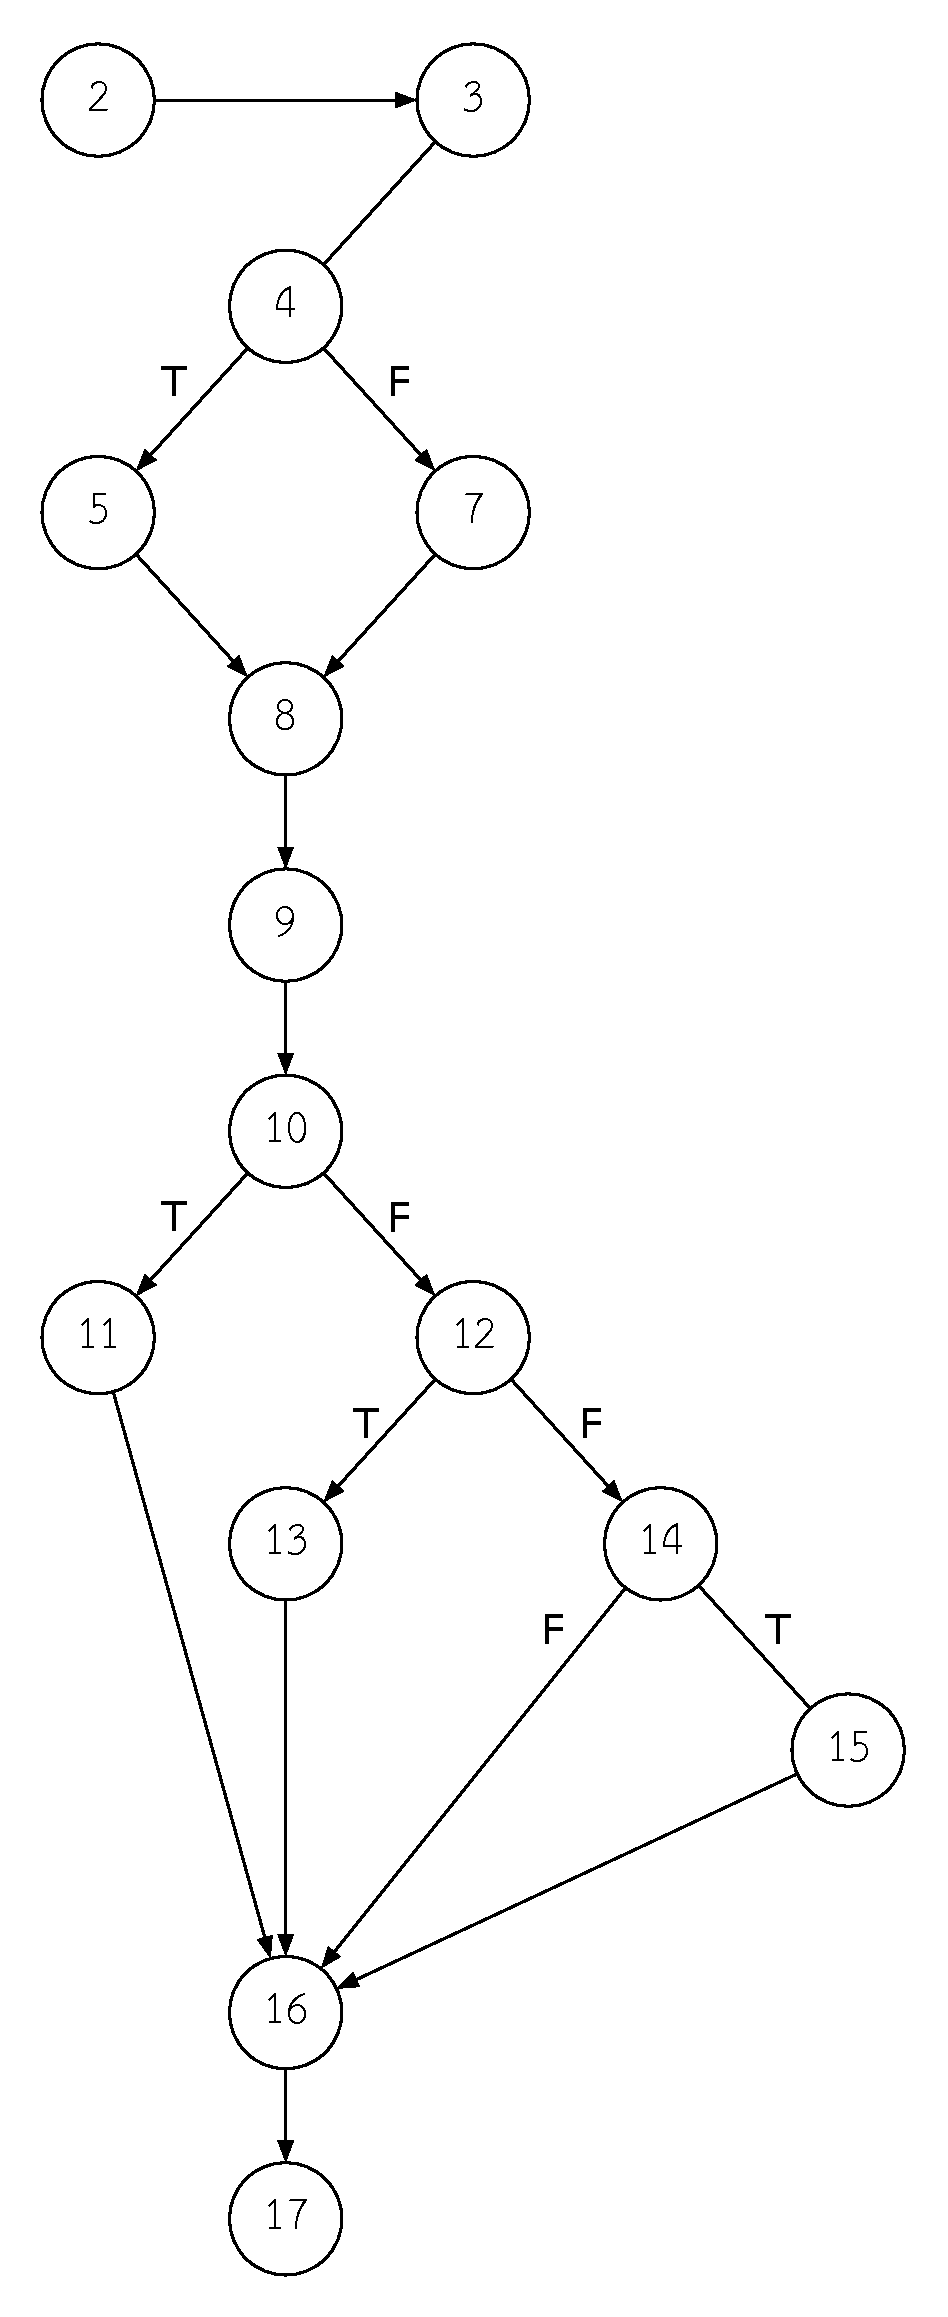
\includegraphics[height=0.65\textheight]{grading-program-graph}
    \caption{กราฟโปรแกรมของชุดรหัสเทียมสำหรับคำนวณเกรดนิสิต}
    \label{fig:programGraph}
\end{figure}

จาก{\figurename} \ref{fig:programGraph} (\pagename\ \pageref{fig:programGraph}) เป็นการนำเสนอชุดรหัสเทียบจาก{\figurename} 
\ref{fig:pseudocodeGrading} ในรูปของกราฟโปรแกรม โดยที่{\Node}ที่ 2-3, 9, 11, 13, 15 และ 17 คือ{\Node}ที่แสดงถึงลำดับการดำเนินงาน 
และ{\Node} 4, 10, 12 และ 14 เป็น{\FirstTimeDefine{\PredicateNode}{\PredicateNodeEN}} ภายในโปรแกรม 
โดยมีโหนด 2 และ 16 เป็น{\FirstTimeDefine{\sourcenode}{\sourcenodeEN}} และ{\FirstTimeDefine{\sinknode}{\sinknodeEN}}ตามลำดับ 
นอกจากรูปแบบความสัมพันธ์ของกราฟโปรแกรมที่แสดงใน{\figurename} \ref{fig:pseudocodeGrading}\ McCabe \cite{Watson1996} 
ได้กำหนดรูปแบบรูปแบบความสัมพันธ์พื้นฐานของกราฟไว้ดัง{\figurename} \ref{fig:graphtype}\ (\pagename\ \pageref{fig:graphtype})

\begin{figure}[ht!]
    \centering
    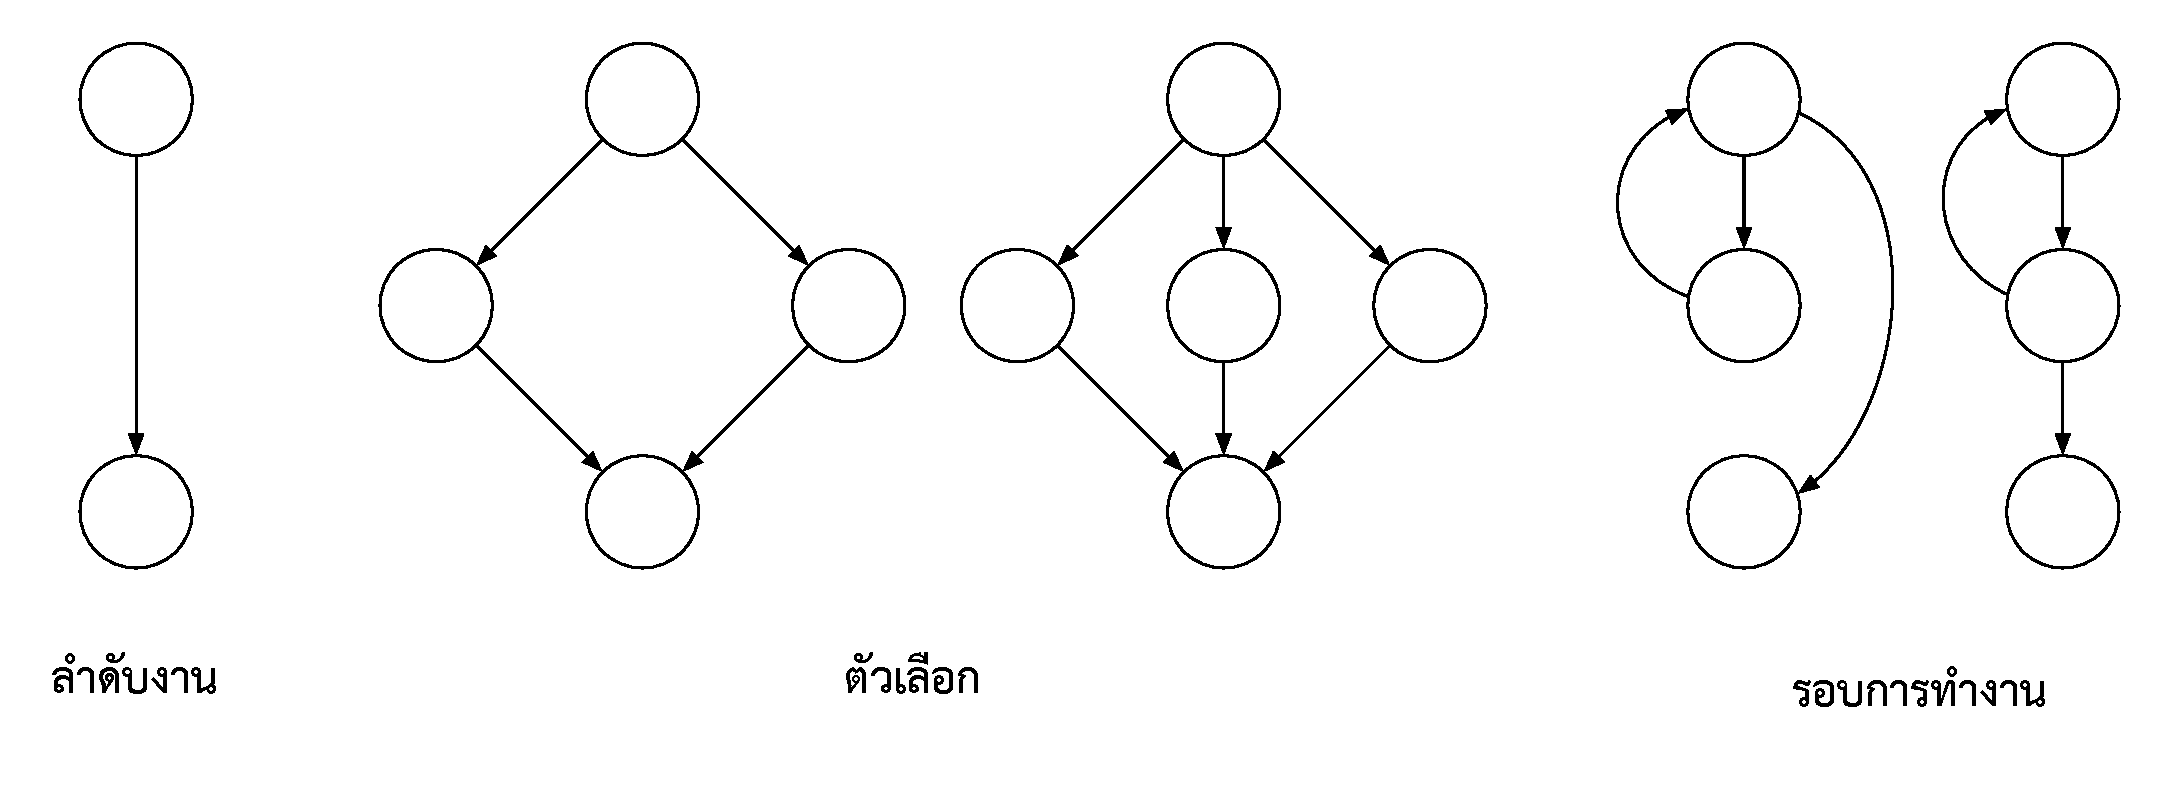
\includegraphics[width=0.9\textwidth]{graph-types}
    \caption{ประเภทของกราฟ}
    \label{fig:graphtype}
\end{figure}

การนำเสนอโปรแกรมในรูปของกราฟโปรแกรมนั้นช่วยให้ผู้ทดสอบวิเคราะห์โครงสร้างของโปรแกรมจากกราฟ 
โดยแยก{\FirstTimeDefine{\BasisPath}{\BasisPathEN}} ทั้งหมดที่เป็นไปได้จากโปรแกรมกราฟ 
โดยแต่ละ{\BasisPath}นั้นจะเริ่มต้นด้วย{\sourcenode}และสิ้นสุดด้วย{\sinknode}เดียวกัน จากนั้นจึงเลือก{\FirstTimeDefine{\TestPath}{\TestPathEN} 
ที่ต้องการทดสอบ แล้วจึงวิเคราะห์{\PredicateNode}ที่ปรากฎบน{\TestPath}ที่เลือก เพื่อสร้างข้อมูลทดสอบที่ทำให้โปรแกรมเรียกใช้งานใน{\TestPath}
ที่เลือกมาได้ ยกตัวอย่างเช่น หากเลือก{\BasisPath}จาก{\figurename} \ref{fig:programGraph}

\begin{figure}[ht!]
    \centering
    \small{$2\ \textendash\ 3\ \textendash\ 
                (4)\ \textendash\ 5\ \textendash\ 8\ \textendash\ 9\ \textendash\ 
                (10)\ \textendash\ 11\ \textendash\ 16\ \textendash\ 17$}
    \caption{ตัวอย่าง{\TestPath}สำหรับโปรแกรมคำนวณเกรด}
    \label{fig:testpath}
\end{figure}
ใช้เป็น{\TestPath} จะพบว่ามี{\PredicateNode}บน{\TestPath}ด้วยกัน 2 {\Node} ด้วยกัน นั่นคือ {\bf 4} และ {\bf 10} 
เมื่อพิจารณา{\PredicateNode}ทั้ง 2 จะได้ข้อมูลทดสอบเป็น {\bf bonus\_score = 50} และ {\bf student\_score = 79} 
ซึ่งข้อมูลทดสอบที่สร้างขึ้นนี้สามารถทำให้โปรแกรมทำงานใน{\TestPath}ได้

\subsection{\FirstTimeDefine{\DDPath}{\DDPathEN}}


% จะเห็นได้ว่าจาก{\figurename} \ref{fig:testpaht} ในขั้นตอนการวิเคราะห์โครงสร้างของโปรแกรมเพื่อสร้างกรณีทดสอบ
% จะสนใจที่{\PredicateNode}ที่โหนด {\bf 4} และ {\bf 10} จึงสามารถลดรูปของโหนดอื่น ๆ ที่เพื่อให้วิเคราะห์ได้ง่ายขึ้น
% ดัง{\figurename} \ref{fig:programGraph}\ จึงสามารถลดรูปลงได้ตามคำจำกัดความของ 
% Decision-to-decision path (DD-Path) \cite{miller1977program}

\begin{enumerate}
    \item[Case 1]: ddd
    \item[Case 2]: ddd
    \item[Case 3]: ddd
    \item[Case 4]: ddd
\end{enumerate}

\subsection{\FirstTimeDefine{\scg}{\scgEN}}
lorem

\subsection{\FirstTimeDefine{\InfeasiblePath}{\InfeasiblePathEN}}
lorem

\subsection{\FirstTimeDefine{\Cyclometric}{\CyclometricEN}}
lorem
